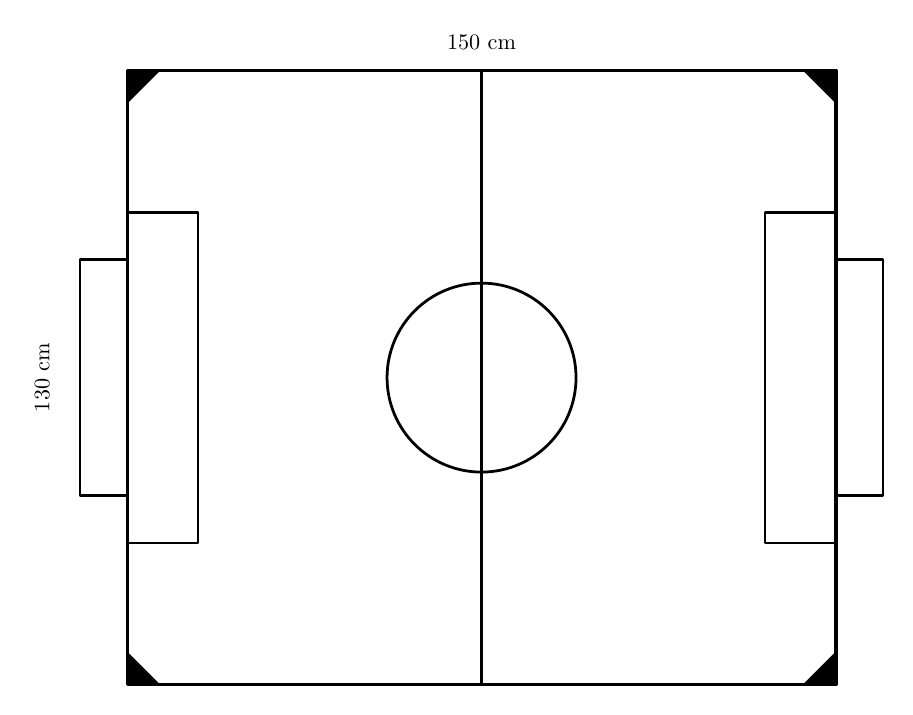
\begin{tikzpicture}[scale=0.06, line cap=round, line join=round]

  % Dimensions: field 150cm x 130cm
  \def\W{150}
  \def\H{130}
  
  % Outer field
  \draw[line width=1.2pt] (0,0) rectangle (\W,\H);
  
  % Chamfered black corners, 7cm
  \foreach \x/\y/\xa/\ya/\xb/\yb in {
  0/0/7/0/0/7,
  150/0/143/0/150/7,
  0/130/7/130/0/123,
  150/130/143/130/150/123}
  {
    \fill (\x,\y) -- (\xa,\ya) -- (\xb,\yb) -- cycle;
  }
  
  % Center line
  \draw[line width=1pt] (75,0) -- (75,\H);
  
  % Center circle, diameter 40cm
  \draw[line width=1pt] (75,65) circle (20);
  
  % Goals
  \draw[line width=1pt] (-10,40) rectangle (0,90);
  \draw[line width=1pt] (\W,40) rectangle (\W+10,90);
  
  % Goal areas / boxes
  \draw[line width=1pt] (0,30) rectangle (15,100);
  \draw[line width=1pt] (\W-15,30) rectangle (\W,100);
  
% --- Penalty arcs via circumcenter / 3 points ---

% Left arc: start (20,55), through (15,65), end (20,75)
\tkzDefPoint(15,55){LA}
\tkzDefPoint(20,65){LB}
\tkzDefPoint(15,75){LC}
\tkzCircumCenter(LA,LB,LC)\tkzGetPoint{LO}
\tkzDrawArc[line width=1pt](LO,LA)(LC)

% Right arc: start (130,75), through (135,65), end (130,55)
\tkzDefPoint(135,75){RA}
\tkzDefPoint(130,65){RB}
\tkzDefPoint(135,55){RC}
\tkzCircumCenter(RA,RB,RC)\tkzGetPoint{RO}
\tkzDrawArc[line width=1pt](RO,RA)(RC)
  
  % Small marks / dots
  % \foreach \x/\y in {
  % 17.5/25, 57.5/25,
  % 17.5/105, 57.5/105,
  % 92.5/25, 132.5/25,
  % 92.5/105, 132.5/105}
  % {
  %   \draw[line width=0.8pt] (\x,\y) circle (1.2);
  % }
  
  % Cross markers
  % \foreach \x/\y/\txt in {
  % 37.5/25/{\textbf{\color{red}(FB)}},
  % 37.5/65/{\textbf{\color{red}(PK, FK)}},
  % 37.5/105/{\textbf{\color{red}(FB)}},
  % 112.5/25/{\textbf{\color{red}(FB)}},
  % 112.5/65/{\textbf{\color{red}(PK, FK)}},
  % 112.5/105/{\textbf{\color{red}(FB)}}}
  % {
  %   \draw[line width=1pt] (\x-2,\y) -- (\x+2,\y);
  %   \draw[line width=1pt] (\x,\y-2) -- (\x,\y+2);
  %   \node[scale=0.75] at (\x,\y+7) {\txt};
  % }
  
  % Optional coordinate labels
  \node[scale=0.8] at (75,136) {150 cm};
  \node[scale=0.8, rotate=90] at (-18,65) {130 cm};
  
  \end{tikzpicture}
